\documentclass[aspectratio=169,10pt]{beamer} % change to aspectratio=43 for 4:3
\usetheme{CLIC}

\usepackage[latin1]{inputenc}
\usepackage[TS1,T1]{fontenc}
\usepackage{lmodern}
\usepackage{xcolor}
\usepackage{graphicx}
\usepackage{multicol}
\usepackage{booktabs}
\usepackage{heppennames2}
\usepackage{multirow}
\usepackage{amsmath}
\usepackage{url}
\usepackage{transparent}
\usepackage[author={test},color=yellow,markup=Highlight]{pdfcomment}

\usepackage{tikz}
\usetikzlibrary{shapes,arrows,positioning}
\usetikzlibrary{backgrounds}
\usetikzlibrary{fit}
\usetikzlibrary{calc}
\tikzstyle{every picture}+=[remember picture]

\usepackage{pgfplots} % LaTeX
\usepgfplotslibrary{groupplots}
\usepackage[european]{circuitikz}
\usepackage[alsoload=hep]{siunitx}

\usetikzlibrary{decorations.pathreplacing}
\newcommand{\tikzmark}[2]{\tikz[remember picture,baseline=(#1.base)]{\node[inner sep=0pt] (#1) {#2};}}
\newcommand{\pt}{p$_{\textnormal{T}}$}

\title[#RELEASE# tracking validation]{\LARGE #RELEASE# tracking validation}
\author[#AUTHORNAME#]{#AUTHORNAME# (#AUTHORINSTITUTE#) \\on behalf of the CLICdp collaboration}
\date[#DATE#]{#DATE#}

% Body
\begin{document}

\frame{
\titlepage 
}

\frame{
\frametitle{Changes from last release}
Full list of changes in \url{https://gitlab.cern.ch/CLICdp/SoftwareConfigurations/iLCSoft/-/releases}
\newline 
\textbf{Package 1}:
\begin{itemize}
\item[-] PR\#0: This changes
\item[-] PR\#1: Other changes
\end{itemize}
}

\frame{
\frametitle{Single Particles: muons}
vs \pt

min number of hits = #MINHITS_SINGLE#
\begin{figure}[bt]
  \centering
  \begin{minipage}[c]{.3\textwidth}
    \centering
    \includegraphics[width=1.0\textwidth]{#PATHPLOTS#/muons/fixedTheta/eff_vs_pt.eps}
  \end{minipage}
  \begin{minipage}[c]{.3\textwidth}
    \centering
    \includegraphics[width=1.0\textwidth]{#PATHPLOTS#/muons/fixedTheta/fake_vs_pt.eps}
  \end{minipage}
  \begin{minipage}[c]{.3\textwidth}
    \centering
    \includegraphics[width=1.0\textwidth]{#PATHPLOTS#/muons/fixedTheta/dupl_vs_pt.eps}
  \end{minipage}
\end{figure}
}

\frame{
\frametitle{Single Particles: muons}
vs $phi$

min number of hits = #MINHITS_SINGLE#
\begin{figure}[bt]
  \centering
  \begin{minipage}[c]{.3\textwidth}
    \centering
    \includegraphics[width=1.0\textwidth]{#PATHPLOTS#/muons/fixedTheta/eff_vs_phi.eps}
  \end{minipage}
  \begin{minipage}[c]{.3\textwidth}
    \centering
    \includegraphics[width=1.0\textwidth]{#PATHPLOTS#/muons/fixedTheta/fake_vs_phi.eps}
  \end{minipage}
  \begin{minipage}[c]{.3\textwidth}
    \centering
    \includegraphics[width=1.0\textwidth]{#PATHPLOTS#/muons/fixedTheta/dupl_vs_phi.eps}
  \end{minipage}
\end{figure}
}


\frame{
\frametitle{Single Particles: muons}
vs $theta$

min number of hits = #MINHITS_SINGLE#
\begin{figure}[bt]
  \centering
  \begin{minipage}[c]{.3\textwidth}
    \centering
    \includegraphics[width=1.0\textwidth]{#PATHPLOTS#/muons/fixedPt/eff_vs_theta.eps}
  \end{minipage}
  \begin{minipage}[c]{.3\textwidth}
    \centering
    \includegraphics[width=1.0\textwidth]{#PATHPLOTS#/muons/fixedPt/fake_vs_theta.eps}
  \end{minipage}
  \begin{minipage}[c]{.3\textwidth}
    \centering
    \includegraphics[width=1.0\textwidth]{#PATHPLOTS#/muons/fixedPt/dupl_vs_theta.eps}
  \end{minipage}
\end{figure}
}

\frame{
\frametitle{Single Particles: muons}
vs $phi$

min number of hits = #MINHITS_SINGLE#
\begin{figure}[bt]
  \centering
  \begin{minipage}[c]{.3\textwidth}
    \centering
    \includegraphics[width=1.0\textwidth]{#PATHPLOTS#/muons/fixedPt/eff_vs_phi.eps}
  \end{minipage}
  \begin{minipage}[c]{.3\textwidth}
    \centering
    \includegraphics[width=1.0\textwidth]{#PATHPLOTS#/muons/fixedPt/fake_vs_phi.eps}
  \end{minipage}
  \begin{minipage}[c]{.3\textwidth}
    \centering
    \includegraphics[width=1.0\textwidth]{#PATHPLOTS#/muons/fixedPt/dupl_vs_phi.eps}
  \end{minipage}
\end{figure}
}

\frame{
\frametitle{Single Particles: electrons}
vs \pt

min number of hits = #MINHITS_SINGLE#
\begin{figure}[bt]
  \centering
  \begin{minipage}[c]{.3\textwidth}
    \centering
    \includegraphics[width=1.0\textwidth]{#PATHPLOTS#/electrons/fixedTheta/eff_vs_pt.eps}
  \end{minipage}
  \begin{minipage}[c]{.3\textwidth}
    \centering
    \includegraphics[width=1.0\textwidth]{#PATHPLOTS#/electrons/fixedTheta/fake_vs_pt.eps}
  \end{minipage}
  \begin{minipage}[c]{.3\textwidth}
    \centering
    \includegraphics[width=1.0\textwidth]{#PATHPLOTS#/electrons/fixedTheta/dupl_vs_pt.eps}
  \end{minipage}
\end{figure}
}

\frame{
\frametitle{Single Particles: electrons}
vs $phi$

min number of hits = #MINHITS_SINGLE#
\begin{figure}[bt]
  \centering
  \begin{minipage}[c]{.3\textwidth}
    \centering
    \includegraphics[width=1.0\textwidth]{#PATHPLOTS#/electrons/fixedTheta/eff_vs_phi.eps}
  \end{minipage}
  \begin{minipage}[c]{.3\textwidth}
    \centering
    \includegraphics[width=1.0\textwidth]{#PATHPLOTS#/electrons/fixedTheta/fake_vs_phi.eps}
  \end{minipage}
  \begin{minipage}[c]{.3\textwidth}
    \centering
    \includegraphics[width=1.0\textwidth]{#PATHPLOTS#/electrons/fixedTheta/dupl_vs_phi.eps}
  \end{minipage}
\end{figure}
}

\frame{
\frametitle{Single Particles: electrons}
vs $theta$

min number of hits = #MINHITS_SINGLE#
\begin{figure}[bt]
  \centering
  \begin{minipage}[c]{.3\textwidth}
    \centering
    \includegraphics[width=1.0\textwidth]{#PATHPLOTS#/electrons/fixedPt/eff_vs_theta.eps}
  \end{minipage}
  \begin{minipage}[c]{.3\textwidth}
    \centering
    \includegraphics[width=1.0\textwidth]{#PATHPLOTS#/electrons/fixedPt/fake_vs_theta.eps}
  \end{minipage}
  \begin{minipage}[c]{.3\textwidth}
    \centering
    \includegraphics[width=1.0\textwidth]{#PATHPLOTS#/electrons/fixedPt/dupl_vs_theta.eps}
  \end{minipage}
\end{figure}
}

\frame{
\frametitle{Single Particles: electrons}
vs $phi$

min number of hits = #MINHITS_SINGLE#
\begin{figure}[bt]
  \centering
  \begin{minipage}[c]{.3\textwidth}
    \centering
    \includegraphics[width=1.0\textwidth]{#PATHPLOTS#/electrons/fixedPt/eff_vs_phi.eps}
  \end{minipage}
  \begin{minipage}[c]{.3\textwidth}
    \centering
    \includegraphics[width=1.0\textwidth]{#PATHPLOTS#/electrons/fixedPt/fake_vs_phi.eps}
  \end{minipage}
  \begin{minipage}[c]{.3\textwidth}
    \centering
    \includegraphics[width=1.0\textwidth]{#PATHPLOTS#/electrons/fixedPt/dupl_vs_phi.eps}
  \end{minipage}
\end{figure}
}

\frame{
\frametitle{Single Particles: pions}
vs \pt

min number of hits = #MINHITS_SINGLE#
\begin{figure}[bt]
  \centering
  \begin{minipage}[c]{.3\textwidth}
    \centering
    \includegraphics[width=1.0\textwidth]{#PATHPLOTS#/pions/fixedTheta/eff_vs_pt.eps}
  \end{minipage}
  \begin{minipage}[c]{.3\textwidth}
    \centering
    \includegraphics[width=1.0\textwidth]{#PATHPLOTS#/pions/fixedTheta/fake_vs_pt.eps}
  \end{minipage}
  \begin{minipage}[c]{.3\textwidth}
    \centering
    \includegraphics[width=1.0\textwidth]{#PATHPLOTS#/pions/fixedTheta/dupl_vs_pt.eps}
  \end{minipage}
\end{figure}
}

\frame{
\frametitle{Single Particles: pions}
vs $phi$

min number of hits = #MINHITS_SINGLE#
\begin{figure}[bt]
  \centering
  \begin{minipage}[c]{.3\textwidth}
    \centering
    \includegraphics[width=1.0\textwidth]{#PATHPLOTS#/pions/fixedTheta/eff_vs_phi.eps}
  \end{minipage}
  \begin{minipage}[c]{.3\textwidth}
    \centering
    \includegraphics[width=1.0\textwidth]{#PATHPLOTS#/pions/fixedTheta/fake_vs_phi.eps}
  \end{minipage}
  \begin{minipage}[c]{.3\textwidth}
    \centering
    \includegraphics[width=1.0\textwidth]{#PATHPLOTS#/pions/fixedTheta/dupl_vs_phi.eps}
  \end{minipage}
\end{figure}
}

\frame{
\frametitle{Single Particles: pions}
vs $theta$

min number of hits = #MINHITS_SINGLE#
\begin{figure}[bt]
  \centering
  \begin{minipage}[c]{.3\textwidth}
    \centering
    \includegraphics[width=1.0\textwidth]{#PATHPLOTS#/pions/fixedPt/eff_vs_theta.eps}
  \end{minipage}
  \begin{minipage}[c]{.3\textwidth}
    \centering
    \includegraphics[width=1.0\textwidth]{#PATHPLOTS#/pions/fixedPt/fake_vs_theta.eps}
  \end{minipage}
  \begin{minipage}[c]{.3\textwidth}
    \centering
    \includegraphics[width=1.0\textwidth]{#PATHPLOTS#/pions/fixedPt/dupl_vs_theta.eps}
  \end{minipage}
\end{figure}
}

\frame{
\frametitle{Single Particles: pions}
vs $theta$

min number of hits = #MINHITS_SINGLE#
\begin{figure}[bt]
  \centering
  \begin{minipage}[c]{.3\textwidth}
    \centering
    \includegraphics[width=1.0\textwidth]{#PATHPLOTS#/pions/fixedPt/eff_vs_theta.eps}
  \end{minipage}
  \begin{minipage}[c]{.3\textwidth}
    \centering
    \includegraphics[width=1.0\textwidth]{#PATHPLOTS#/pions/fixedPt/fake_vs_theta.eps}
  \end{minipage}
  \begin{minipage}[c]{.3\textwidth}
    \centering
    \includegraphics[width=1.0\textwidth]{#PATHPLOTS#/pions/fixedPt/dupl_vs_theta.eps}
  \end{minipage}
\end{figure}
}

\frame{
\frametitle{Complex events: ttbar3TeV}
vs \pt

min number of hits = #MINHITS_COMPLEX#
\begin{figure}[bt]
  \centering
  \begin{minipage}[c]{.3\textwidth}
    \centering
    \includegraphics[width=1.0\textwidth]{#PATHPLOTS#/ttbar3TeV/eff_vs_pt.eps}
  \end{minipage}
  \begin{minipage}[c]{.3\textwidth}
    \centering
    \includegraphics[width=1.0\textwidth]{#PATHPLOTS#/ttbar3TeV/fake_vs_pt.eps}
  \end{minipage}
  \begin{minipage}[c]{.3\textwidth}
    \centering
    \includegraphics[width=1.0\textwidth]{#PATHPLOTS#/ttbar3TeV/dupl_vs_pt.eps}
  \end{minipage}
\end{figure}
}

\frame{
\frametitle{Complex events: ttbar3TeV}
vs $theta$

min number of hits = #MINHITS_COMPLEX#
\begin{figure}[bt]
  \centering
  \begin{minipage}[c]{.3\textwidth}
    \centering
    \includegraphics[width=1.0\textwidth]{#PATHPLOTS#/ttbar3TeV/eff_vs_theta.eps}
  \end{minipage}
  \begin{minipage}[c]{.3\textwidth}
    \centering
    \includegraphics[width=1.0\textwidth]{#PATHPLOTS#/ttbar3TeV/fake_vs_theta.eps}
  \end{minipage}
  \begin{minipage}[c]{.3\textwidth}
    \centering
    \includegraphics[width=1.0\textwidth]{#PATHPLOTS#/ttbar3TeV/dupl_vs_theta.eps}
  \end{minipage}
\end{figure}
}

\frame{
\frametitle{Complex events: ttbar3TeV}
vs $phi$

min number of hits = #MINHITS_COMPLEX#
\begin{figure}[bt]
  \centering
  \begin{minipage}[c]{.3\textwidth}
    \centering
    \includegraphics[width=1.0\textwidth]{#PATHPLOTS#/ttbar3TeV/eff_vs_phi.eps}
  \end{minipage}
  \begin{minipage}[c]{.3\textwidth}
    \centering
    \includegraphics[width=1.0\textwidth]{#PATHPLOTS#/ttbar3TeV/fake_vs_phi.eps}
  \end{minipage}
  \begin{minipage}[c]{.3\textwidth}
    \centering
    \includegraphics[width=1.0\textwidth]{#PATHPLOTS#/ttbar3TeV/dupl_vs_phi.eps}
  \end{minipage}
\end{figure}
}


\clicSplashWhite

\end{document}
